\appendix
\chapter{Параметры дыхательной системы} 
\begin{table}[!ht]
    \centering
    \begin{tabular}{|p{1.5in}|p{1.5in}|p{1.5in}|}
    \hline 
    \textbf{Символ} & \textbf{Значение} & \textbf{Размерность} \\ \hline 
    $\rho $ & 1.23e-6 & ${kg\mathord{\left/ {\vphantom {kg cm^{3} }} \right. \kern-\nulldelimiterspace} cm^{3} } $ \\ \hline 
    $\eta $ & 1.8e-3 & ${kg\mathord{\left/ {\vphantom {kg \left(cm\; s\right)}} \right. \kern-\nulldelimiterspace} \left(cm\; s\right)} $ \\ \hline 
    $\theta _{O_{2} } $ & 0.17 & $cm^{2} /s$ \\ \hline 
    $\theta _{CO_{2} } $ & 0.16 & $cm^{2} /s$ \\ \hline 
    $D_{O_{2} } $ & 1.2e-3 & ${l\mathord{\left/ {\vphantom {l s}} \right. \kern-\nulldelimiterspace} s} $ \\ \hline 
    $D_{CO_{2} } $ & 6.7e-2 & ${l\mathord{\left/ {\vphantom {l s}} \right. \kern-\nulldelimiterspace} s} $ \\ \hline 
    $E_{a} $ & 0.5 & ${kPa\mathord{\left/ {\vphantom {kPa l}} \right. \kern-\nulldelimiterspace} l} $ \\ \hline 
    $\nu $\textit{} & 0.16 & $Hz$ \\ \hline 
    $V_{a,0} $\textit{} & 0.625 & $l$ \\ \hline 
    $p_{g} $ & 1.3 & $kPa$ \\ \hline 
    $p_{atm} $ & 101.3 & $kPa$ \\ \hline 
    $V_{blood} $ & 4 & $l$ \\ \hline 
    $V_{minute} $ & 5 & $l$ \\ \hline 
    $Q_{O_{2} }^{b} $ & 0.25 & ${l\mathord{\left/ {\vphantom {l \min }} \right. \kern-\nulldelimiterspace} \min } $ \\ \hline 
    $Q_{_{CO_{2} } }^{b} $ & 0.2 & ${l\mathord{\left/ {\vphantom {l \min }} \right. \kern-\nulldelimiterspace} \min } $ \\ \hline 
    $C_{O_{2} }^{atm} $ & 0.209 &  \\ \hline 
    $C_{CO_{2} }^{atm} $ & 2.8e-4 &  \\ \hline 
    $T_{pt} $ & 1 & $\min $ \\ \hline 
    \end{tabular}
    \caption{Константы модели дыхательной системы}
    \label{tab:langPuram}
\end{table}


\begin{table}
    \caption{Параметры 1D структуры трахейно-бронхиального дерева}
    \centering
    \begin{tabular}{|p{0.7in}|p{1.5in}|p{1.5in}|p{1.0in}|} \hline 
    \textbf{Индекс} & \textbf{Длина, }$cm$ & \textbf{Диаметр, }$cm$\textbf{} & $c_{0} ,\; {cm\mathord{\left/ {\vphantom {cm s}} \right. \kern-\nulldelimiterspace} s} $\textbf{} \\ \hline 
    1 & 12.49 & 1.38 & 7700 \\ \hline 
    2 & 5.41 & 0.87 & 7382 \\ \hline 
    3 & 2.86 & 1.11 & 7382 \\ \hline 
    4 & 1.25 & 0.68 & 7064 \\ \hline 
    5 & 1.63 & 0.66 & 7064 \\ \hline 
    6 & 2.45 & 0.84 & 7064 \\ \hline 
    7 & 1.82 & 0.53 & 7064 \\ \hline 
    8 & 2.32 & 0.25 & 6747 \\ \hline 
    9 & 1.5 & 0.47 & 6747 \\ \hline 
    10 & 3.86 & 0.26 & 6747 \\ \hline 
    11 & 1.02 & 0.43 & 6747 \\ \hline 
    12 & 2.1 & 0.44 & 6747 \\ \hline 
    13 & 0.6 & 0.64 & 6747 \\ \hline 
    14 & 0.54 & 0.4 & 6747 \\ \hline 
    15 & 1,29 & 0.27 & 6747 \\ \hline 
    \end{tabular}
    \label{tab:lang1d}
\end{table}

\begin{table}[!ht]
	\centering
	\caption{Константы модели регуляции дыхания.}
	\medskip
	\label{tab:params_reg}
	\begin{tabular}{|c|c|c|}
		\hline
		Символ & Значение & Размерность \\
		\hline
		\(V_{SS}\)& 5 & л\slash мин \\
		\hline
		\(K_{cCO_{2}}\) & 0.4& л\slash (мин*мм рт. ст.) \\
		\hline
		\(T_{cCO_{2}}\) & 48.4 & мм рт. ст. \\
		\hline
		\(K_{pCO_{2}}\) & 0.25 & л\slash (мин*мм рт. ст.) \\
		\hline
		\(T_{pCO_{2}}\) & 38.7 & мм рт. ст. \\
		\hline
		\(\alpha\) & 0.152&  \\
		\hline
		\(\beta\) & 0.683 &  \\
		\hline
		\(V_{E,T}\) & 15& л\slash мин\\
		\hline
		\(\tau\) & 250 & сек\\
		\hline
	\end{tabular}
\end{table}

\chapter{Параметры кровеносной системы} 
\begin{table}[!ht]
\centering
\caption{Параметры модели баланса газов в крови}
\medskip
\label{tabular:tab3}
\begin{tabular}{|c|c|c|}
\hline
Символ & Значение & Размерность \\
\hline
\(m\) & 3.6 &  \\
\hline
\(T_{Hb}\) & 2.66e-3 & моль\slash л \\
\hline
\(\sigma_{O_{2}}\) & 1.18e-6 & моль\slash (л*мм рт. ст.) \\
\hline
\(V_{b}\) & 6 & л \\
\hline
\(K_{O_{2}}\) & 2.1e-6 & л\slash моль\\
\hline
\( \dot{V}_{O_{2}}\) & 0.28 & л\slash мин \\
\hline
\(K_{CO_{2}}\) & 7.425e-7& \\
\hline
\(M\) & 2.04e-2& моль\slash л \\
\hline
\end{tabular}
\end{table}

\chapter{Графики моделирования тестов с возрастающей нагрузкой}
\label{AppendixС}

\begin{figure}[!ht]
	\centering
	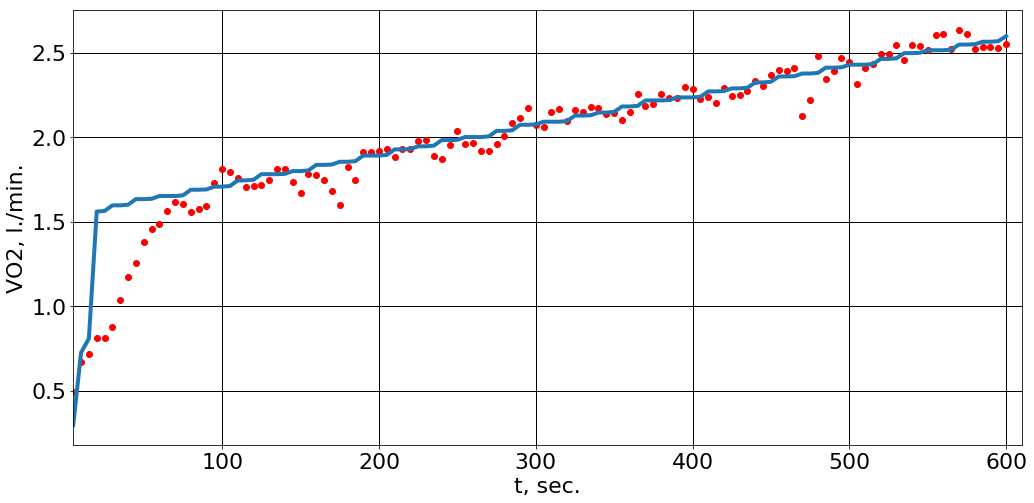
\includegraphics[scale=0.25]{sp11.png}
	\caption{Спортсмен S1. Сравнение экспериментальных и расчетных показателей потребления кислорода } 
\end{figure}

\begin{figure}[!ht]
	\centering
	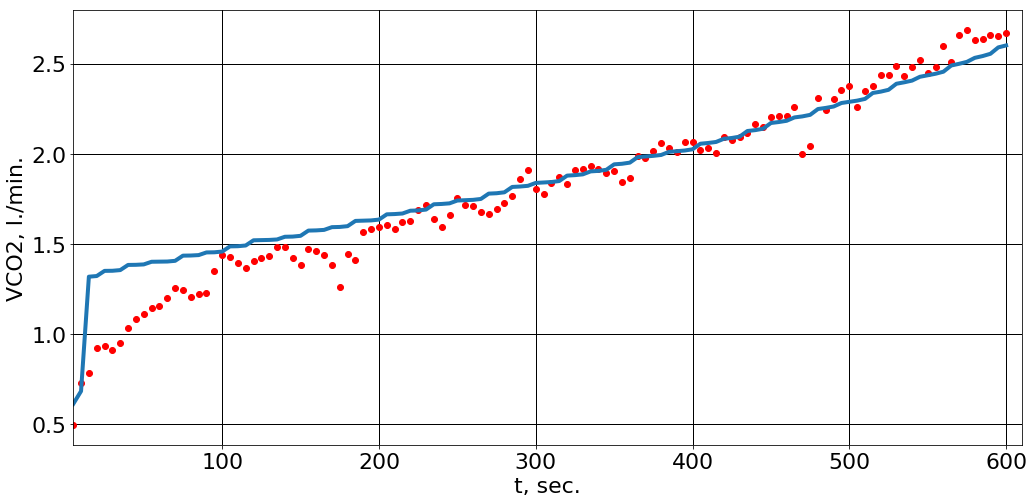
\includegraphics[scale=0.25]{sp12.png}
	\caption{Спортсмен S1. Сравнение экспериментальных и расчетных показателей выделения углекислого газа} 
\end{figure}

\begin{figure}[!ht]
	\centering
	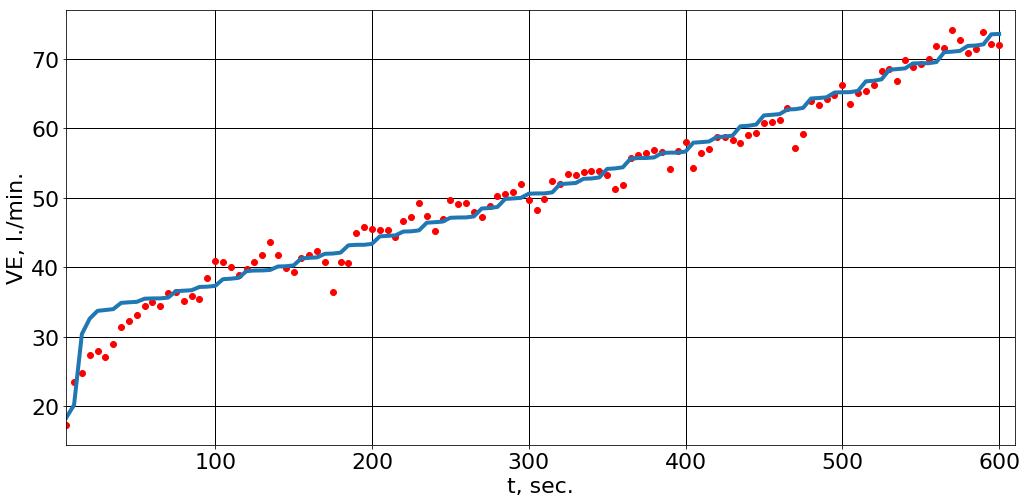
\includegraphics[scale=0.25]{sp14.png}
	\caption{Спортсмен S1. Сравнение экспериментальных и расчетных показателей минутной вентиляции легких} 
\end{figure}

\begin{figure}[!ht]
	\centering
	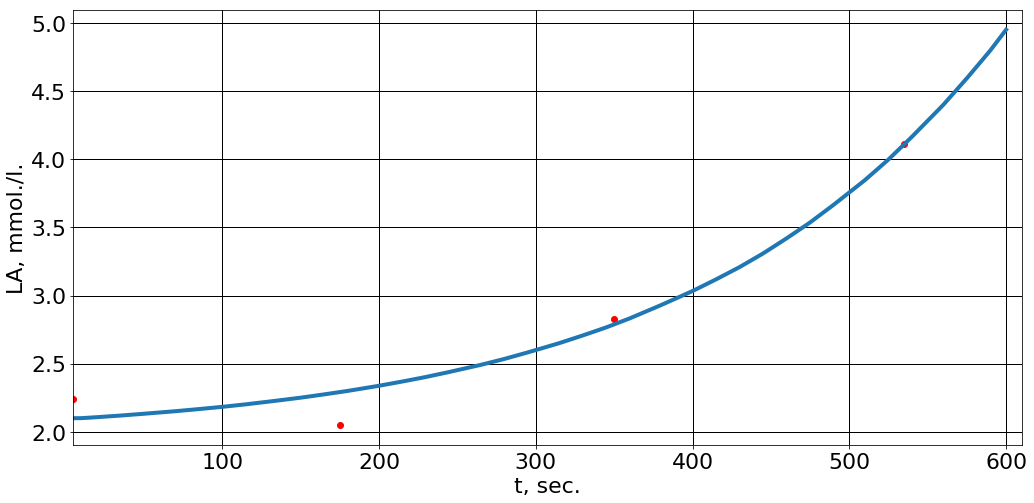
\includegraphics[scale=0.25]{sp13.png}
	\caption{Спортсмен S1. Сравнение экспериментальных и расчетных показателей концентрации лактата} 
\end{figure}

\begin{figure}[!ht]
	\centering
	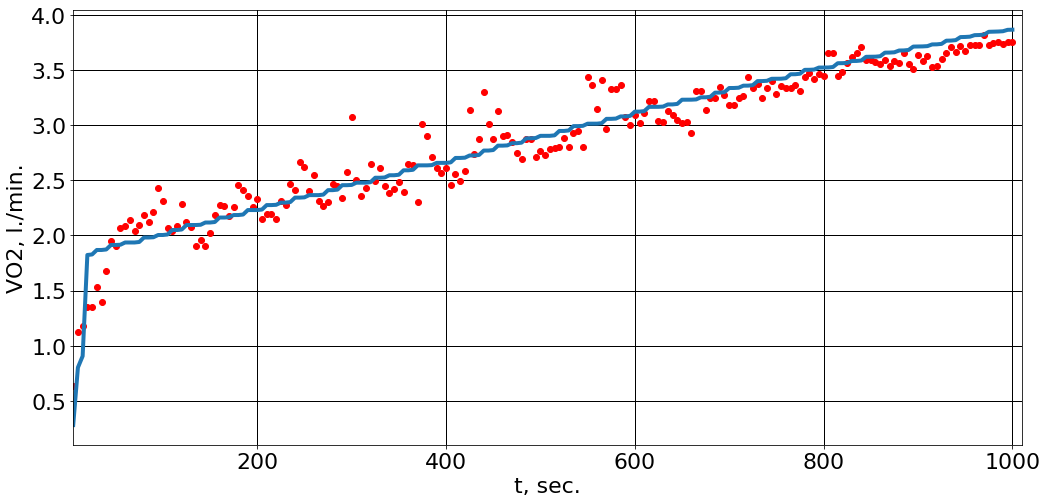
\includegraphics[scale=0.25]{sp21.png}
	\caption{Спортсмен S2. Сравнение экспериментальных и расчетных показателей потребления кислорода } 
\end{figure}

\begin{figure}[!ht]
	\centering
	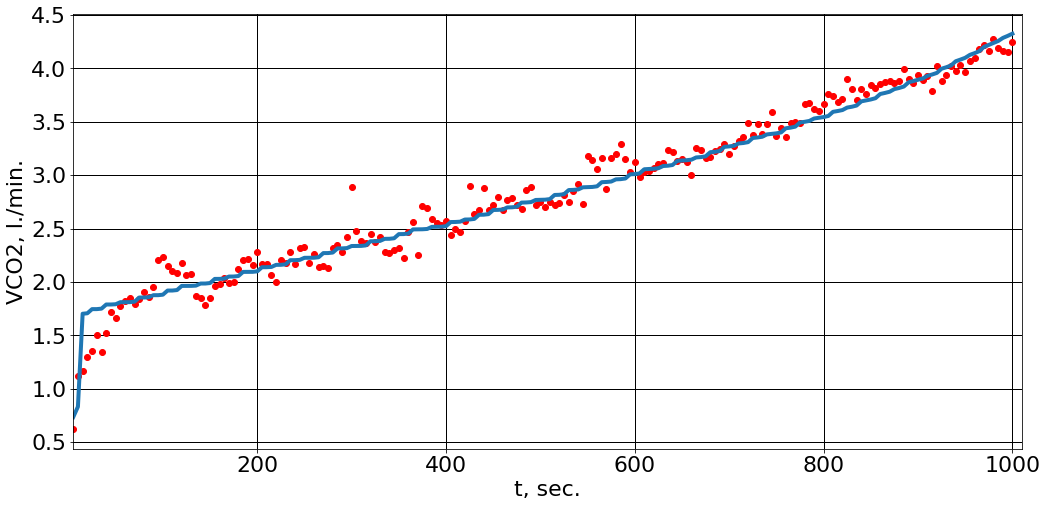
\includegraphics[scale=0.25]{sp22.png}
	\caption{Спортсмен S2. Сравнение экспериментальных и расчетных показателей выделения углекислого газа} 
\end{figure}

\begin{figure}[!ht]
	\centering
	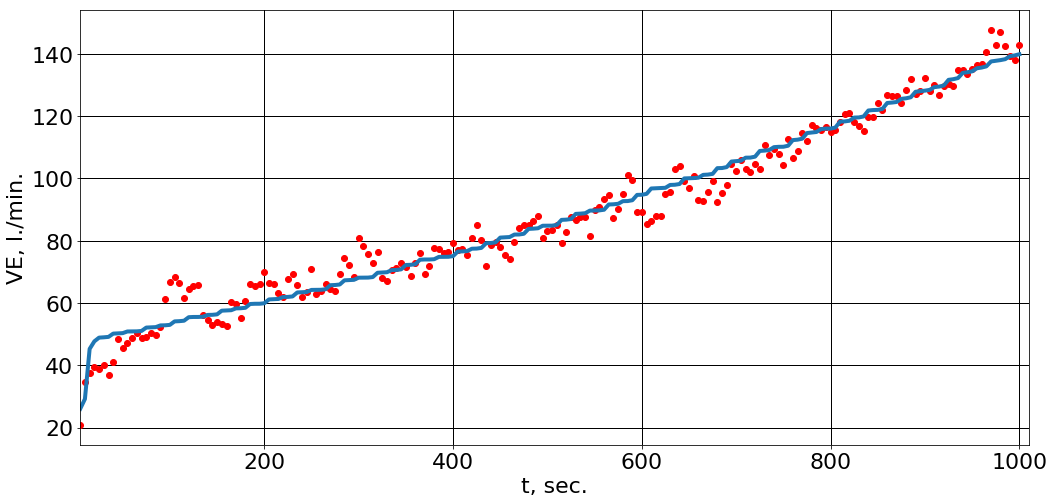
\includegraphics[scale=0.25]{sp24.png}
	\caption{Спортсмен S2. Сравнение экспериментальных и расчетных показателей минутной вентиляции легких} 
\end{figure}

\begin{figure}[!ht]
	\centering
	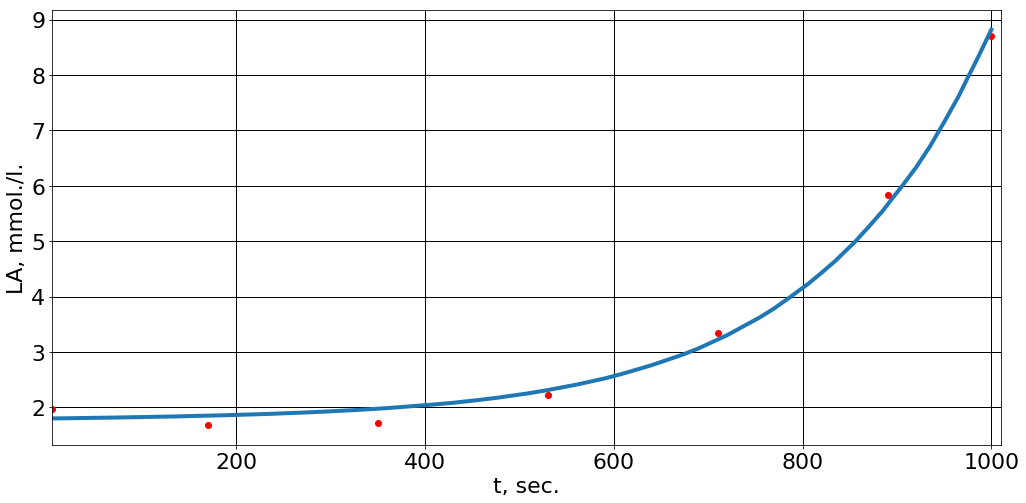
\includegraphics[scale=0.25]{sp23.png}
	\caption{Спортсмен S2. Сравнение экспериментальных и расчетных показателей концентрации лактата} 
\end{figure}

\begin{figure}[!ht]
	\centering
	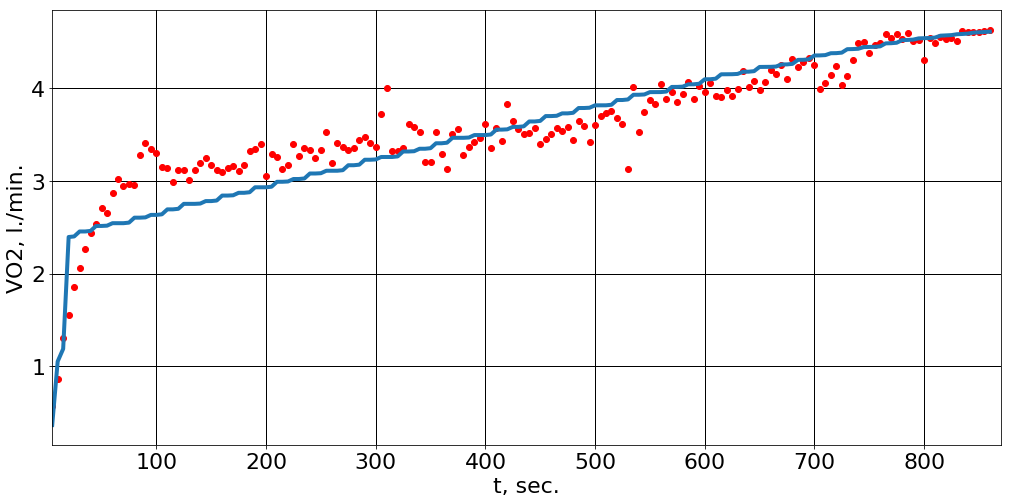
\includegraphics[scale=0.25]{sp31.png}
	\caption{Спортсмен S3. Сравнение экспериментальных и расчетных показателей потребления кислорода } 
\end{figure}

\begin{figure}[!ht]
	\centering
	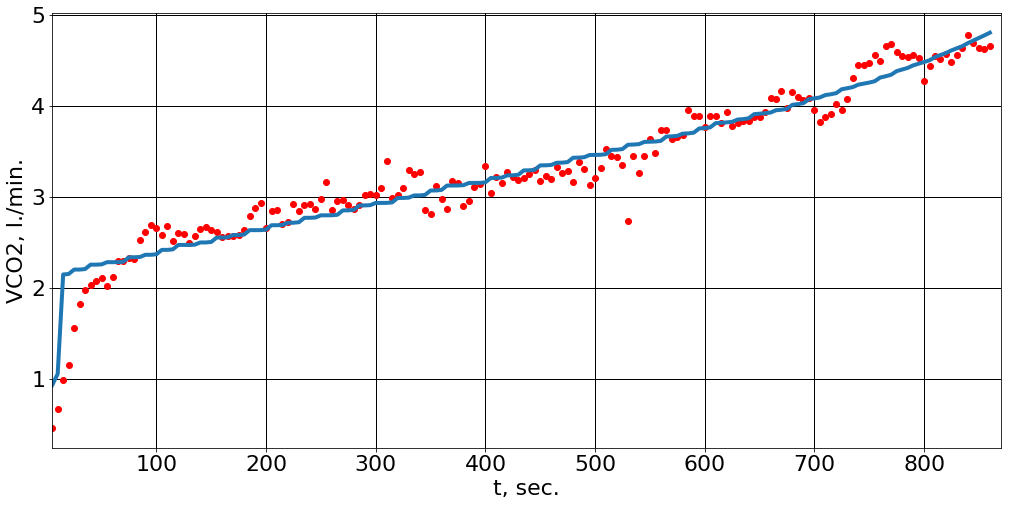
\includegraphics[scale=0.25]{sp32.png}
	\caption{Спортсмен S3. Сравнение экспериментальных и расчетных показателей выделения углекислого газа} 
\end{figure}

\begin{figure}[!ht]
	\centering
	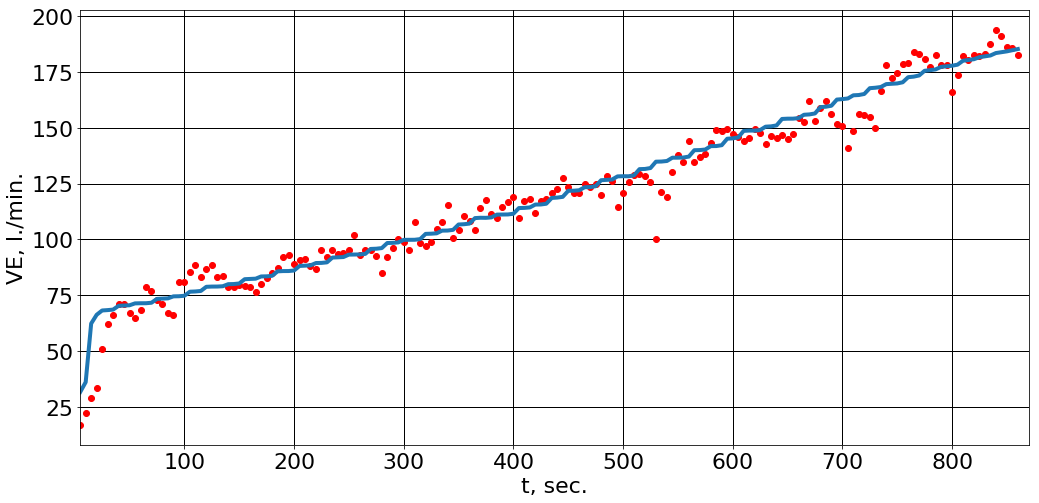
\includegraphics[scale=0.25]{sp34.png}
	\caption{Спортсмен S3. Сравнение экспериментальных и расчетных показателей минутной вентиляции легких} 
\end{figure}

\begin{figure}[!ht]
	\centering
	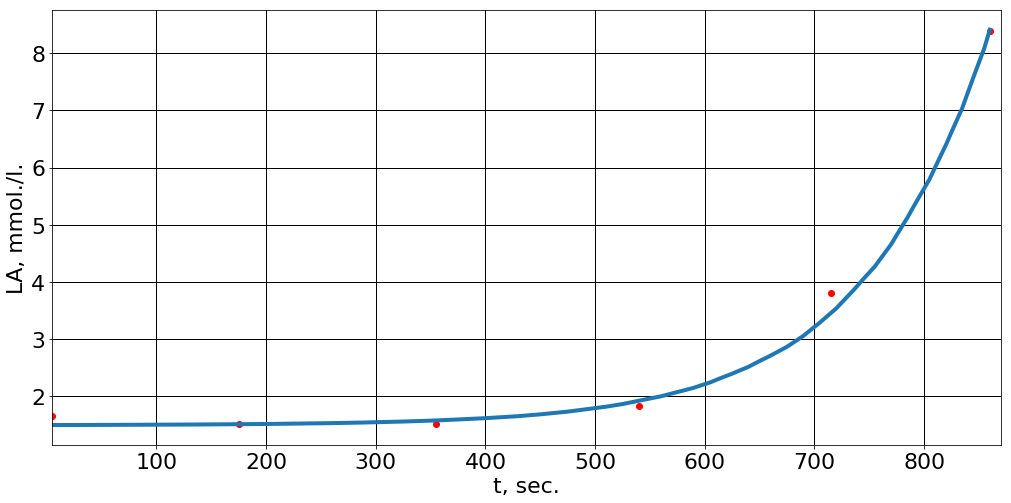
\includegraphics[scale=0.25]{sp33.png}
	\caption{Спортсмен S3. Сравнение экспериментальных и расчетных показателей концентрации лактата} 
\end{figure}

\begin{figure}[!ht]
	\centering
	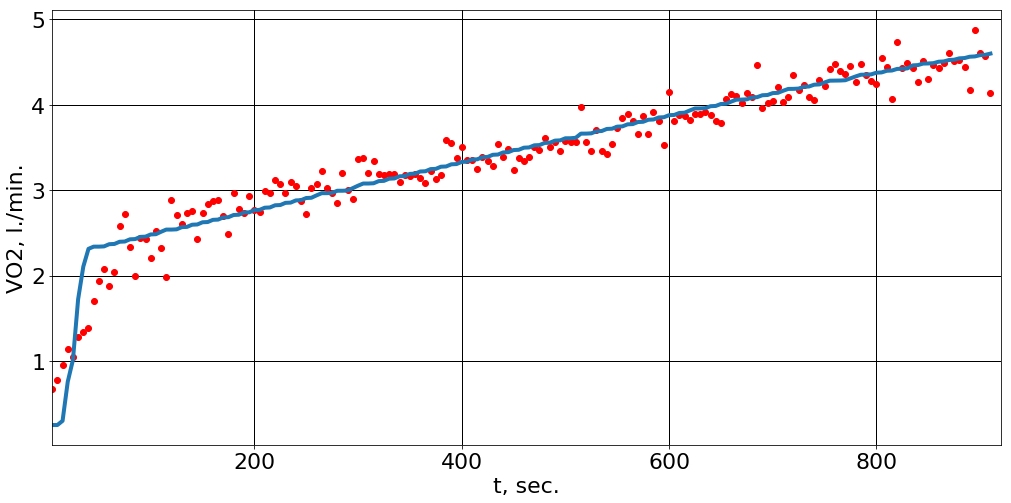
\includegraphics[scale=0.25]{sp41.png}
	\caption{Спортсмен S4. Сравнение экспериментальных и расчетных показателей потребления кислорода } 
\end{figure}

\begin{figure}[!ht]
	\centering
	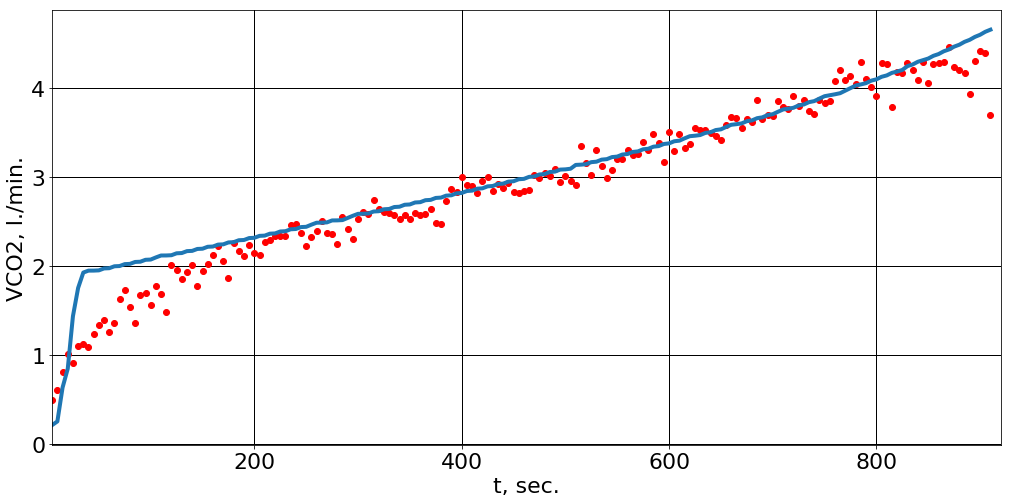
\includegraphics[scale=0.25]{sp42.png}
	\caption{Спортсмен S4. Сравнение экспериментальных и расчетных показателей выделения углекислого газа} 
\end{figure}

\begin{figure}[!ht]
	\centering
	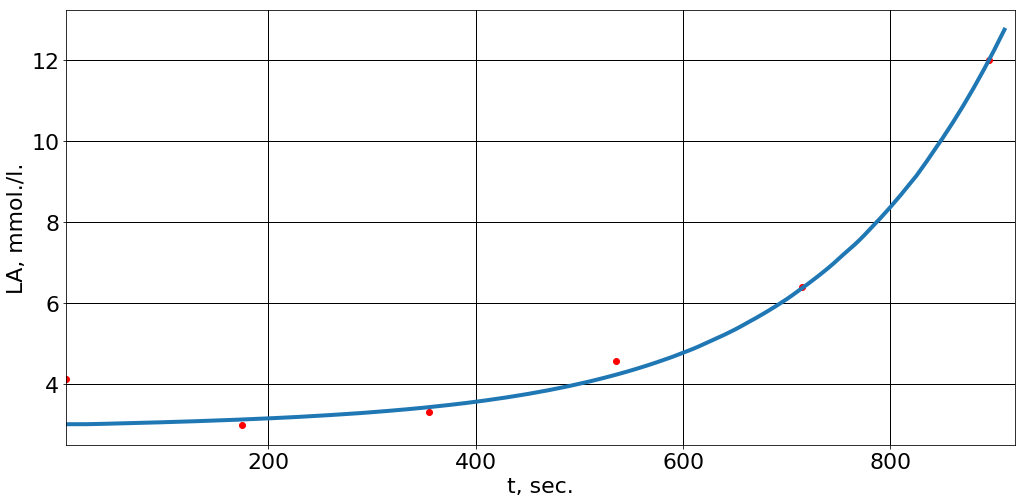
\includegraphics[scale=0.25]{sp43.png}
	\caption{Спортсмен S4. Сравнение экспериментальных и расчетных показателей минутной вентиляции легких} 
\end{figure}

\begin{figure}[!ht]
	\centering
	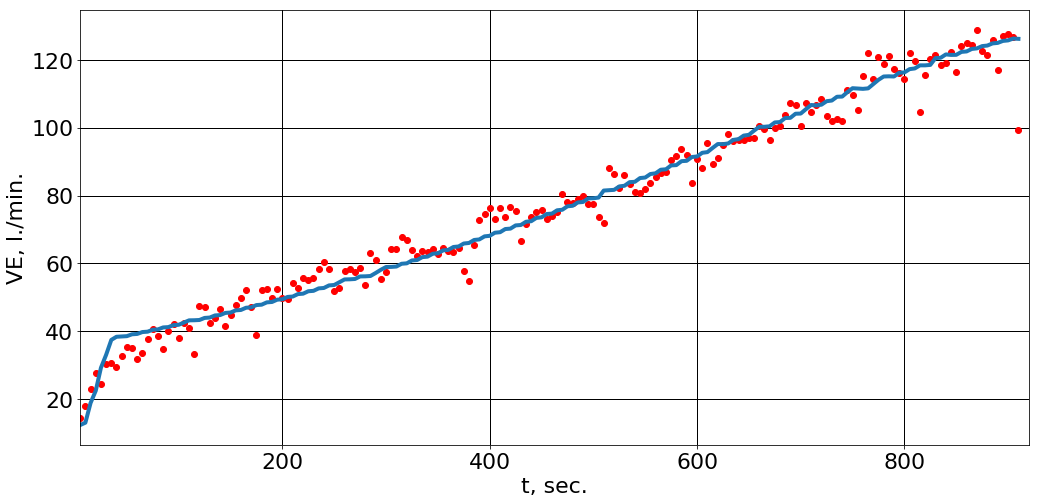
\includegraphics[scale=0.25]{sp44.png}
	\caption{Спортсмен S4. Сравнение экспериментальных и расчетных показателей концентрации лактата} 
\end{figure}

\begin{figure}[!ht]
	\centering
	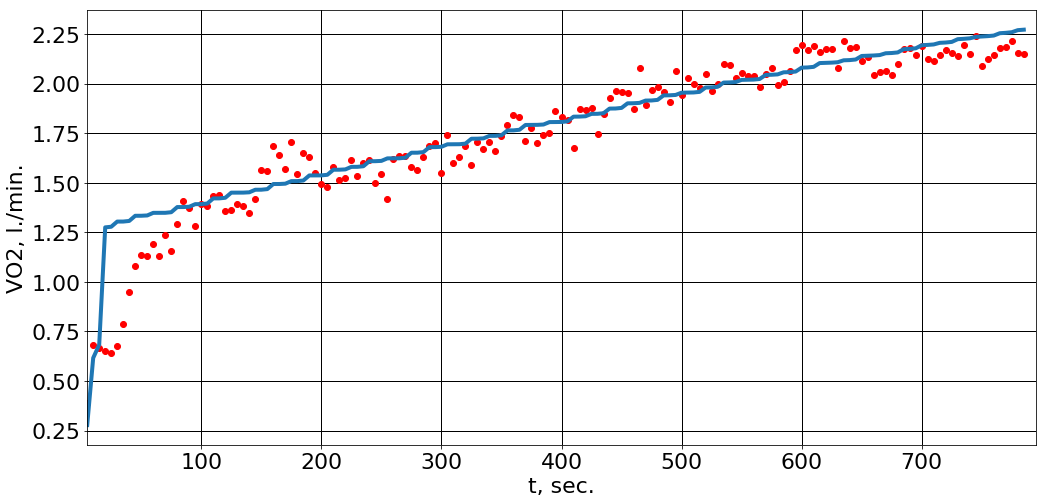
\includegraphics[scale=0.25]{sp51.png}
	\caption{Спортсмен S5. Сравнение экспериментальных и расчетных показателей потребления кислорода } 
\end{figure}

\begin{figure}[!ht]
	\centering
	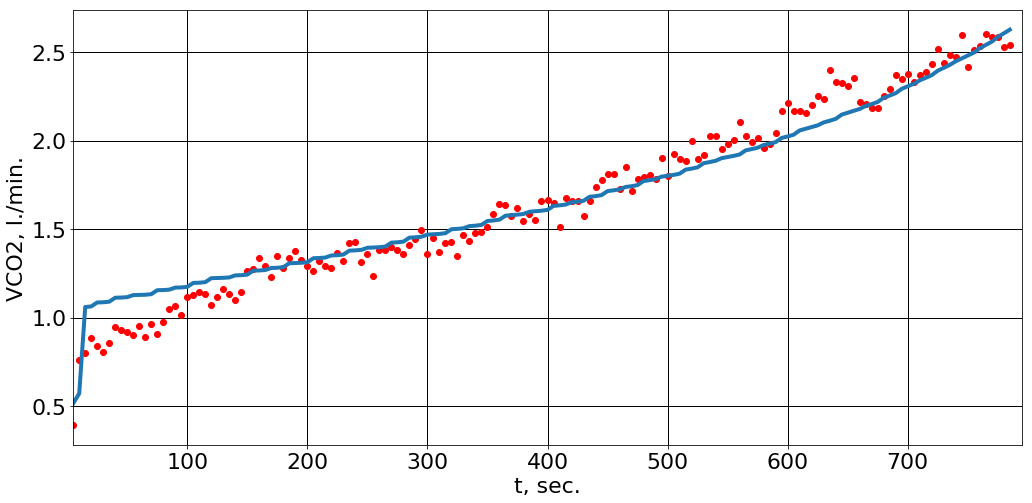
\includegraphics[scale=0.25]{sp52.png}
	\caption{Спортсмен S5. Сравнение экспериментальных и расчетных показателей выделения углекислого газа} 
\end{figure}

\begin{figure}[!ht]
	\centering
	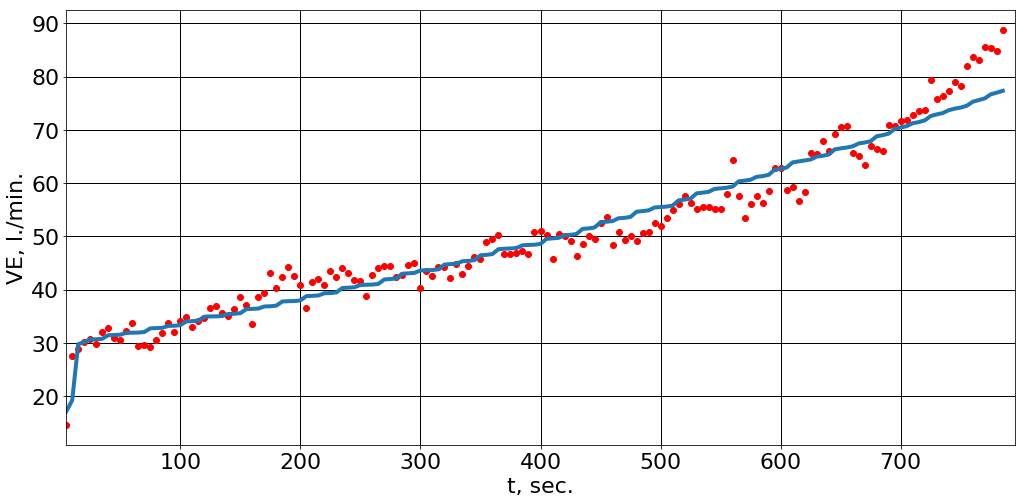
\includegraphics[scale=0.25]{sp54.png}
	\caption{Спортсмен S5. Сравнение экспериментальных и расчетных показателей минутной вентиляции легких} 
\end{figure}

\begin{figure}[!ht]
	\centering
	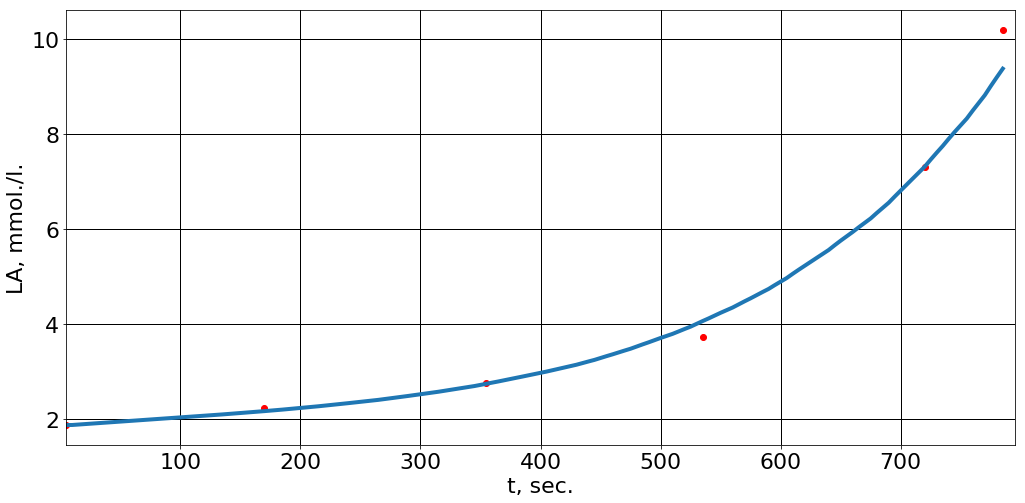
\includegraphics[scale=0.25]{sp53.png}
	\caption{Спортсмен S5. Сравнение экспериментальных и расчетных показателей концентрации лактата} 
\end{figure}

\begin{figure}[!ht]
	\centering
	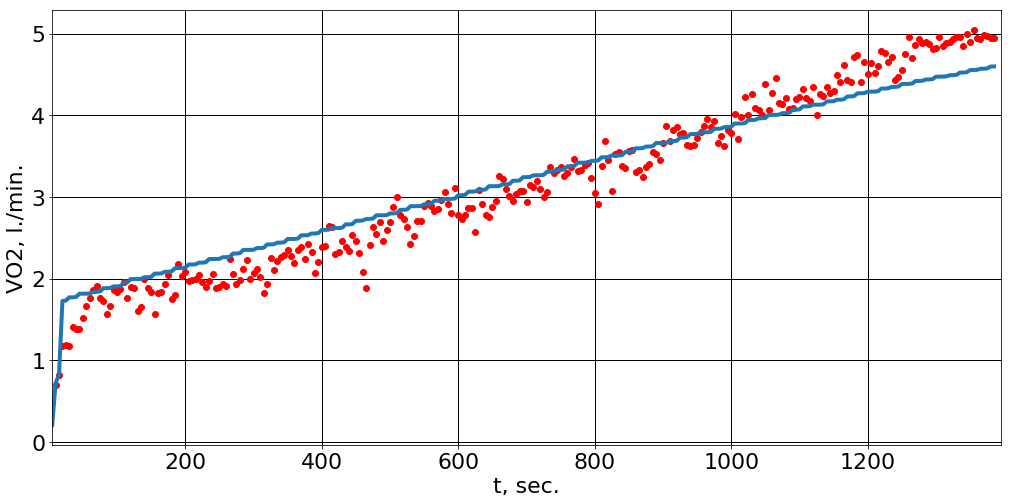
\includegraphics[scale=0.25]{sp61.png}
	\caption{Спортсмен S6. Сравнение экспериментальных и расчетных показателей потребления кислорода } 
\end{figure}

\begin{figure}[!ht]
	\centering
	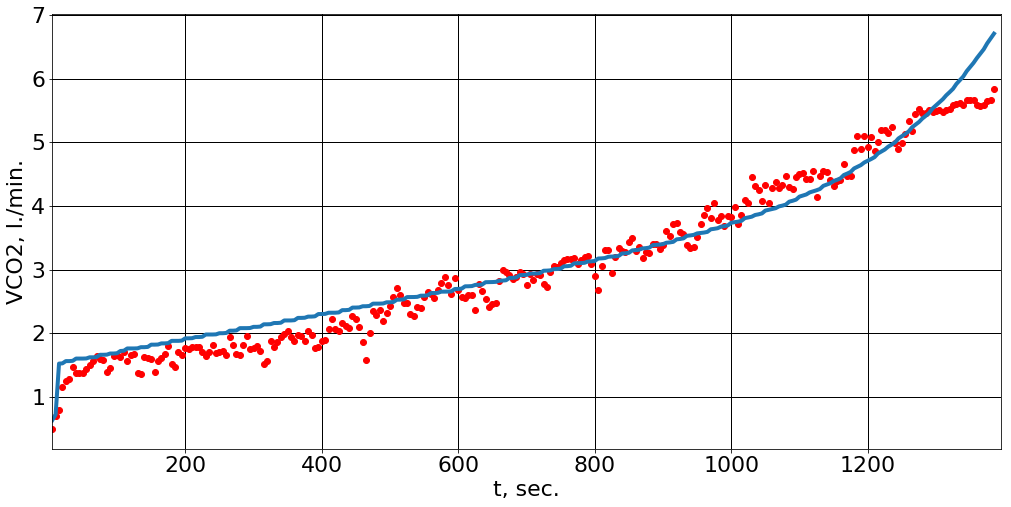
\includegraphics[scale=0.25]{sp62.png}
	\caption{Спортсмен S6. Сравнение экспериментальных и расчетных показателей выделения углекислого газа} 
\end{figure}

\begin{figure}[!ht]
	\centering
	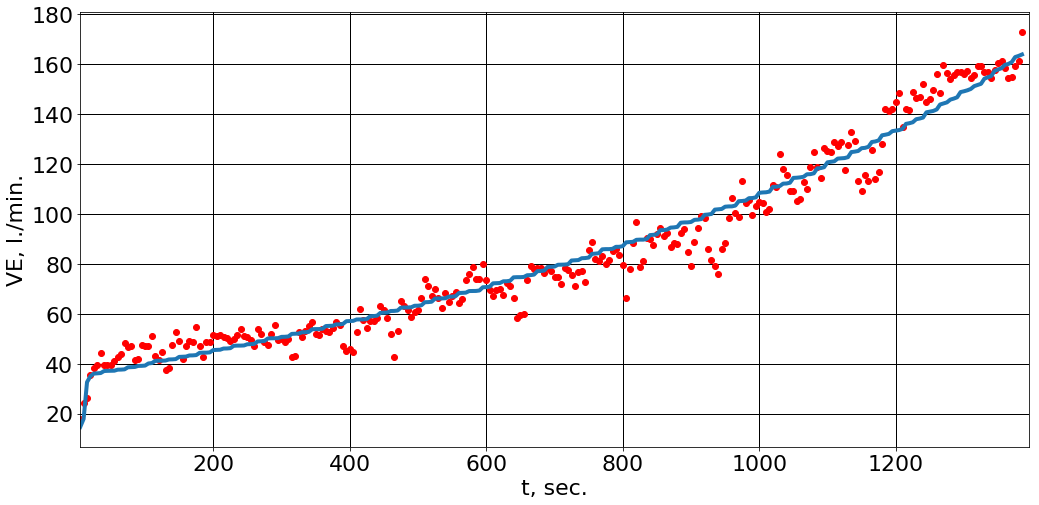
\includegraphics[scale=0.25]{sp64.png}
	\caption{Спортсмен S6. Сравнение экспериментальных и расчетных показателей минутной вентиляции легких} 
\end{figure}

\begin{figure}[!ht]
	\centering
	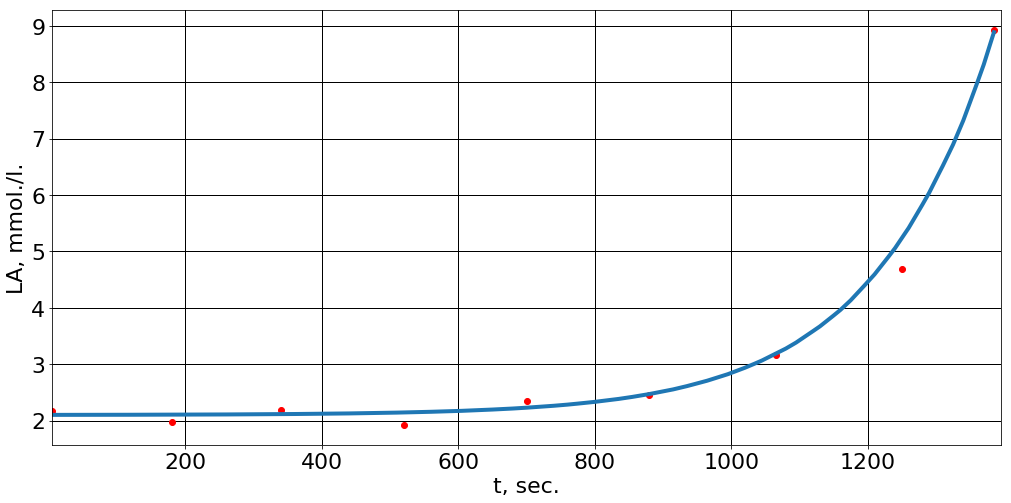
\includegraphics[scale=0.25]{sp63.png}
	\caption{Спортсмен S6. Сравнение экспериментальных и расчетных показателей концентрации лактата} 
\end{figure}

\begin{figure}[!ht]
	\centering
	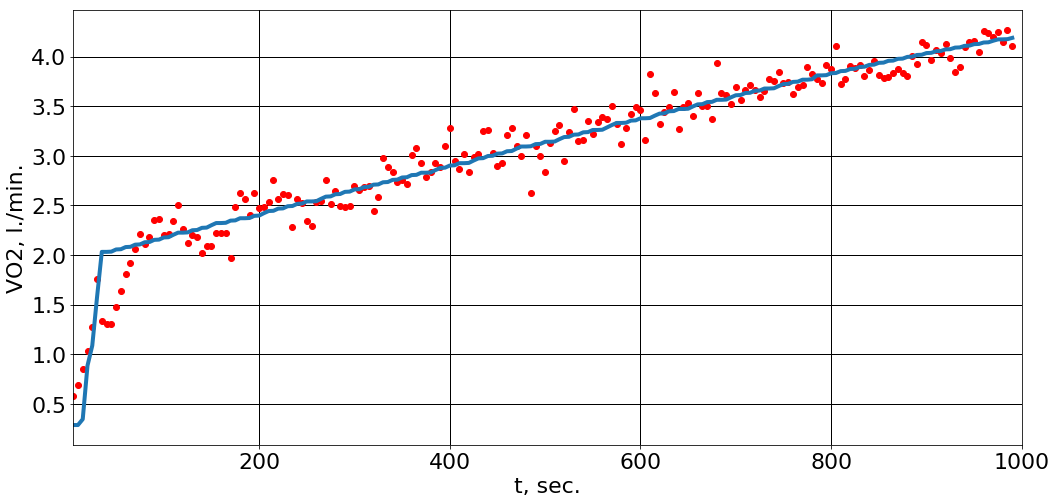
\includegraphics[scale=0.25]{sp71.png}
	\caption{Спортсмен S7. Сравнение экспериментальных и расчетных показателей потребления кислорода } 
\end{figure}

\begin{figure}[!ht]
	\centering
	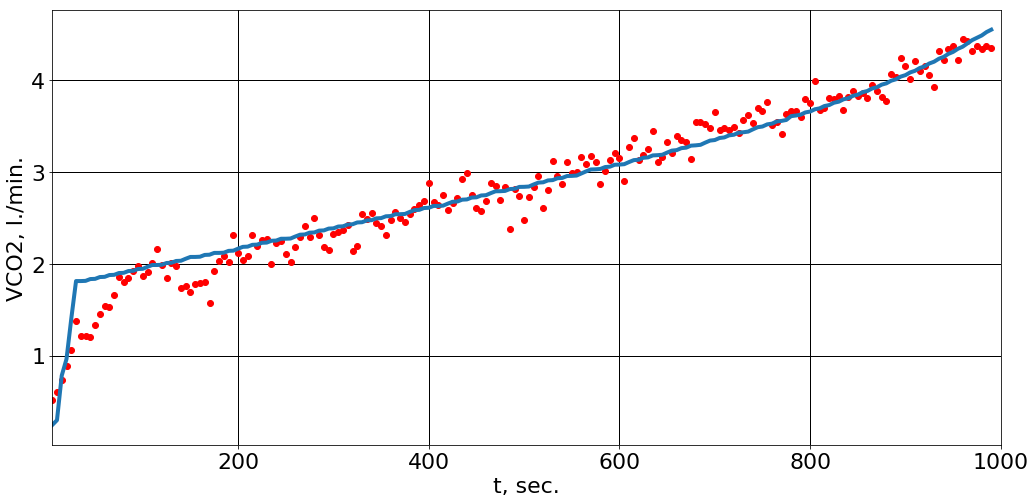
\includegraphics[scale=0.25]{sp72.png}
	\caption{Спортсмен S7. Сравнение экспериментальных и расчетных показателей выделения углекислого газа} 
\end{figure}

\begin{figure}[!ht]
	\centering
	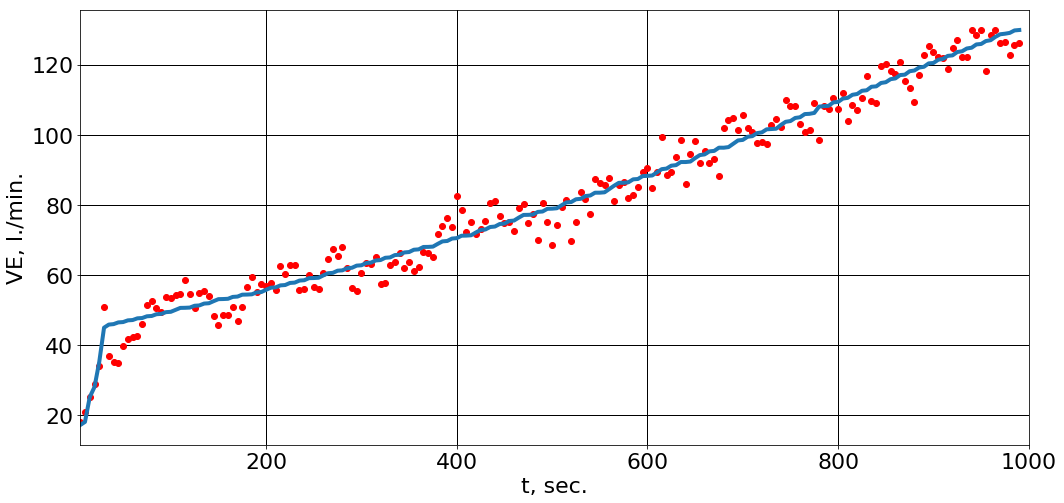
\includegraphics[scale=0.25]{sp74.png}
	\caption{Спортсмен S7. Сравнение экспериментальных и расчетных показателей минутной вентиляции легких} 
\end{figure}

\begin{figure}[!ht]
	\centering
	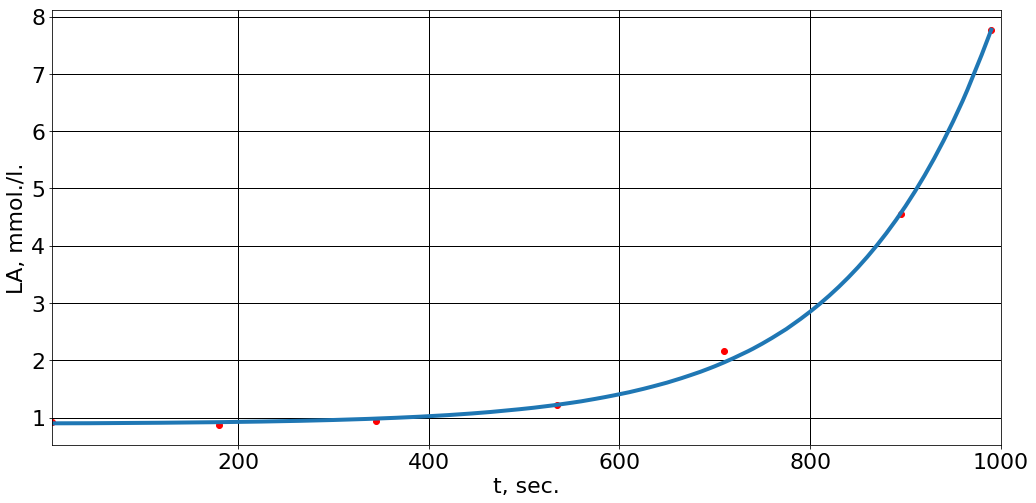
\includegraphics[scale=0.25]{sp73.png}
	\caption{Спортсмен S7. Сравнение экспериментальных и расчетных показателей концентрации лактата} 
\end{figure}

\begin{figure}[!ht]
	\centering
	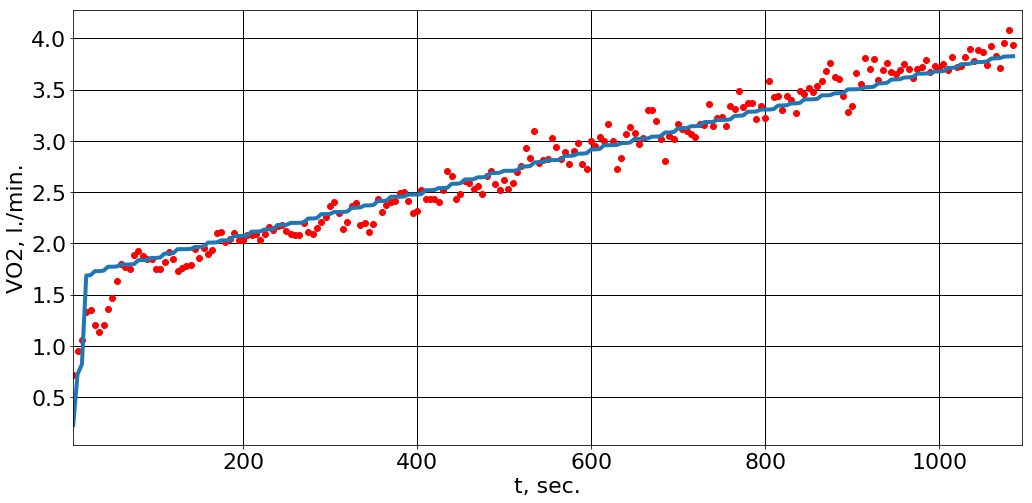
\includegraphics[scale=0.25]{sp81.png}
	\caption{Спортсмен S8. Сравнение экспериментальных и расчетных показателей потребления кислорода } 
\end{figure}

\begin{figure}[!ht]
	\centering
	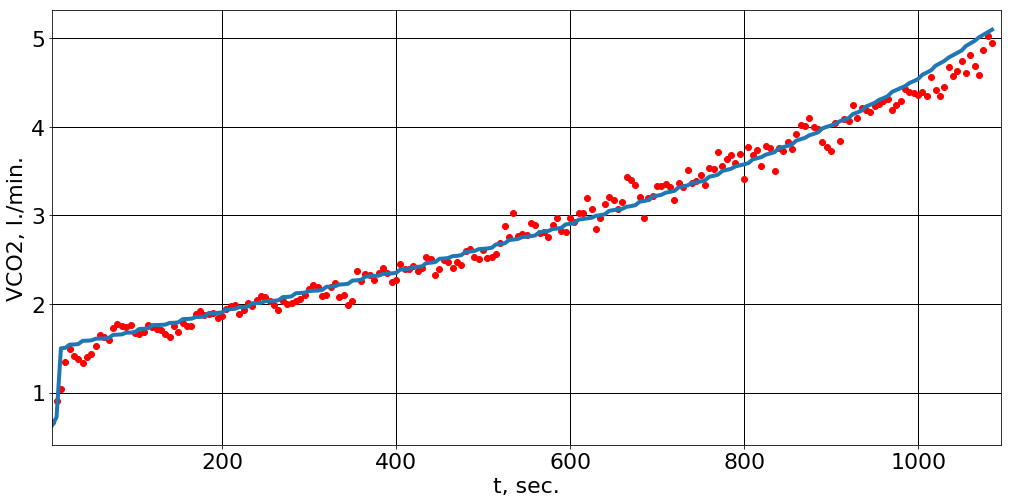
\includegraphics[scale=0.25]{sp82.png}
	\caption{Спортсмен S8. Сравнение экспериментальных и расчетных показателей выделения углекислого газа} 
\end{figure}

\begin{figure}[!ht]
	\centering
	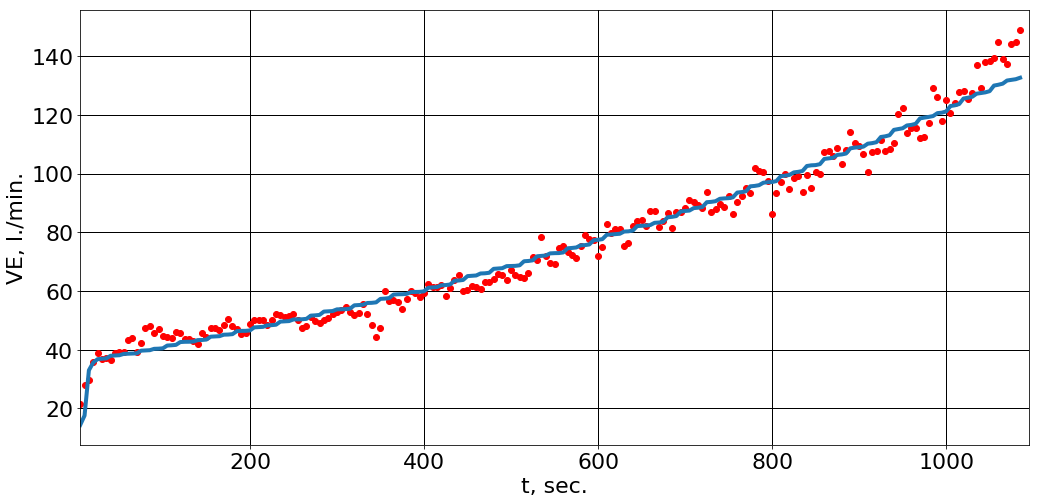
\includegraphics[scale=0.25]{sp84.png}
	\caption{Спортсмен S8. Сравнение экспериментальных и расчетных показателей минутной вентиляции легких} 
\end{figure}

\begin{figure}[!ht]
	\centering
	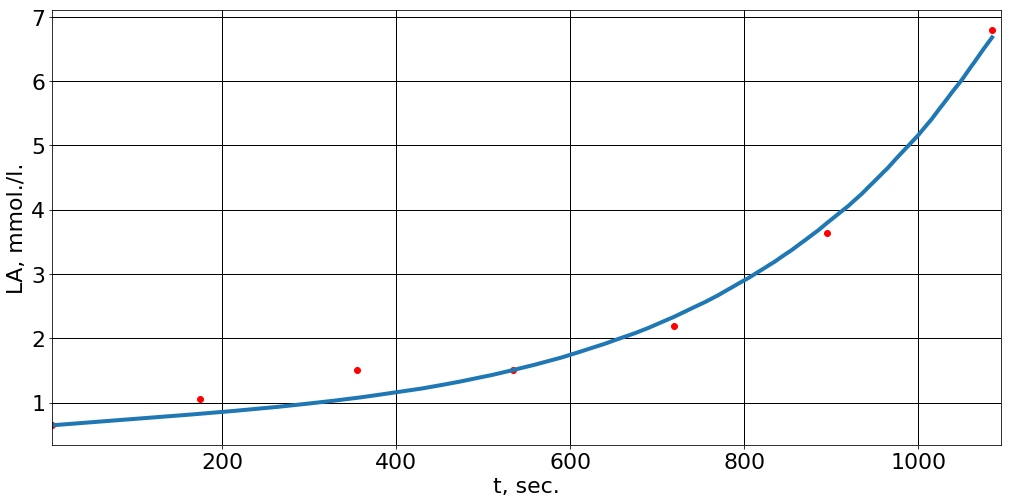
\includegraphics[scale=0.25]{sp83.png}
	\caption{Спортсмен S8. Сравнение экспериментальных и расчетных показателей концентрации лактата} 
\end{figure}

\begin{figure}[!ht]
	\centering
	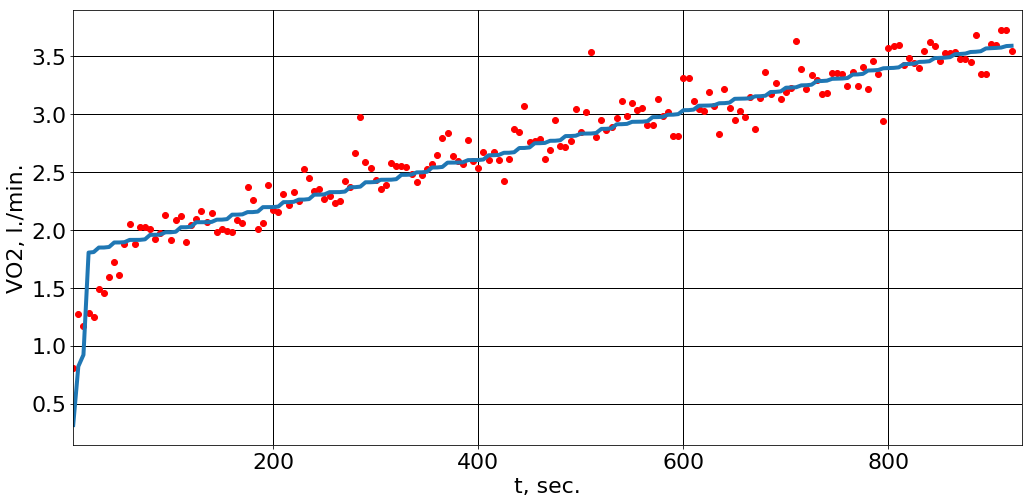
\includegraphics[scale=0.25]{sp91.png}
	\caption{Спортсмен S9. Сравнение экспериментальных и расчетных показателей потребления кислорода } 
\end{figure}

\begin{figure}[!ht]
	\centering
	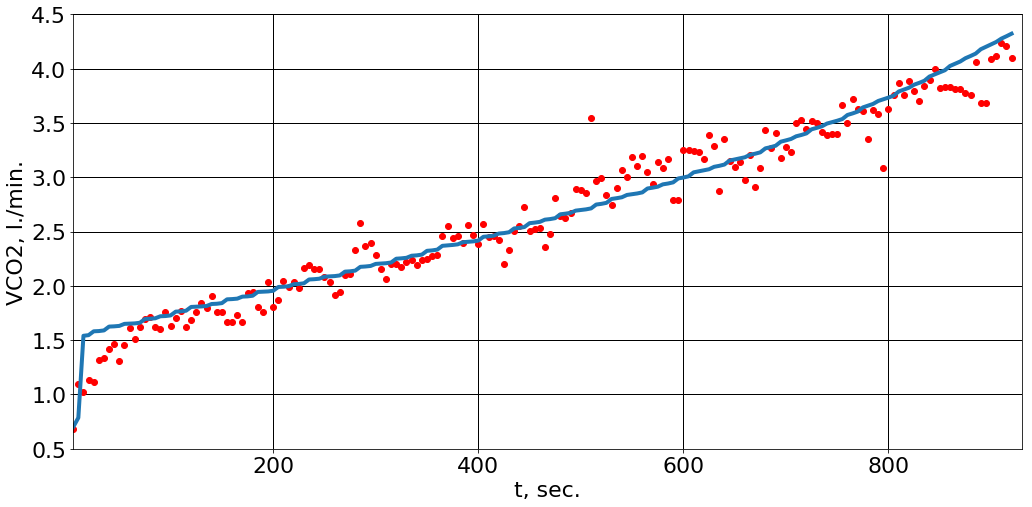
\includegraphics[scale=0.25]{sp92.png}
	\caption{Спортсмен S9. Сравнение экспериментальных и расчетных показателей выделения углекислого газа} 
\end{figure}

\begin{figure}[!ht]
	\centering
	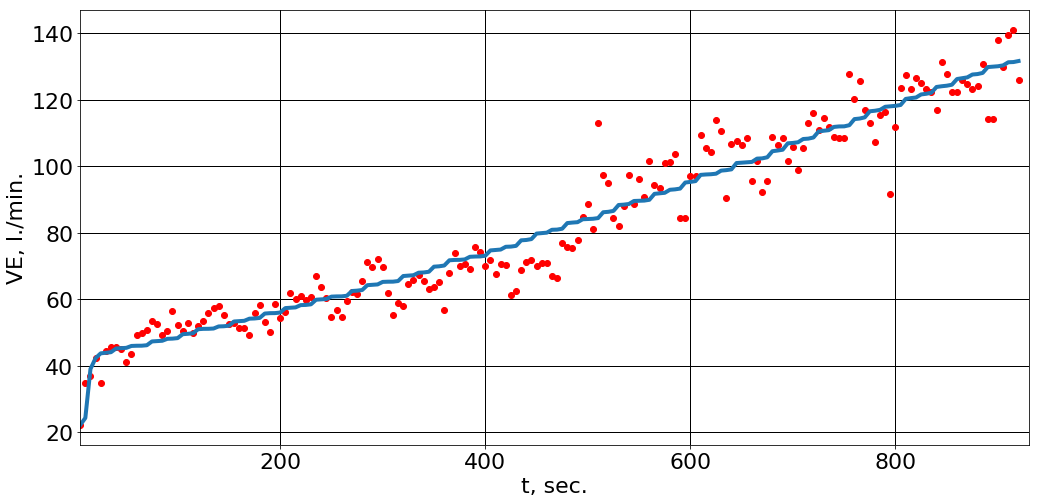
\includegraphics[scale=0.25]{sp94.png}
	\caption{Спортсмен S9. Сравнение экспериментальных и расчетных показателей минутной вентиляции легких} 
\end{figure}

\begin{figure}[!ht]
	\centering
	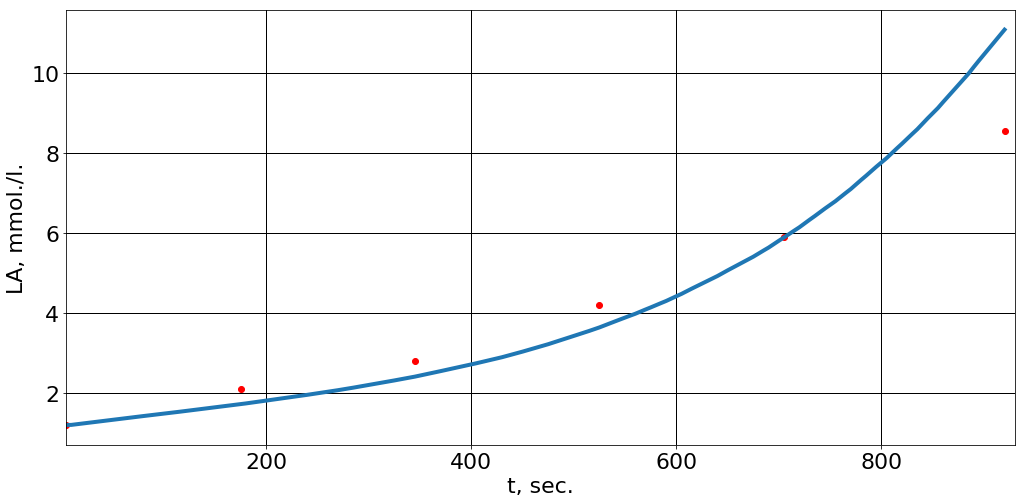
\includegraphics[scale=0.25]{sp93.png}
	\caption{Спортсмен S9. Сравнение экспериментальных и расчетных показателей концентрации лактата} 
\end{figure}

\begin{figure}[!ht]
	\centering
	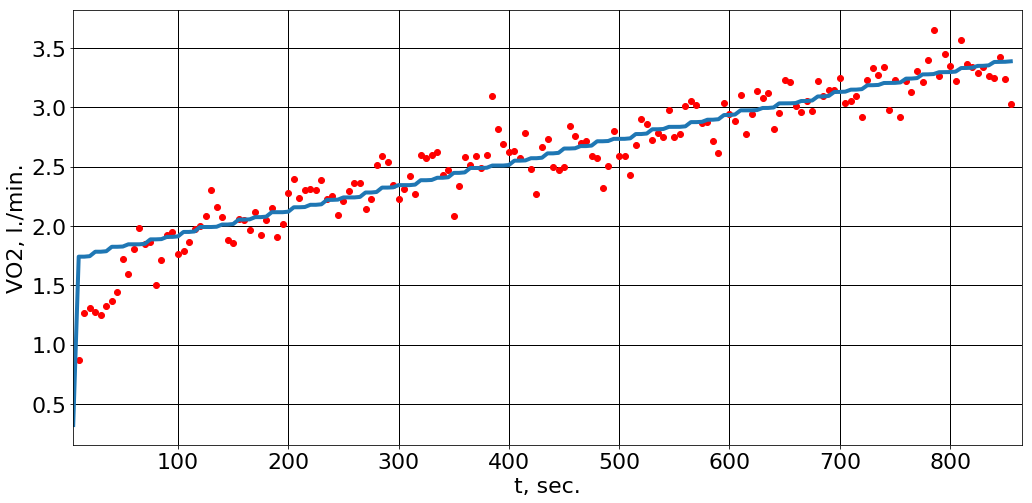
\includegraphics[scale=0.25]{sp101.png}
	\caption{Спортсмен S10. Сравнение экспериментальных и расчетных показателей потребления кислорода } 
\end{figure}

\begin{figure}[!ht]
	\centering
	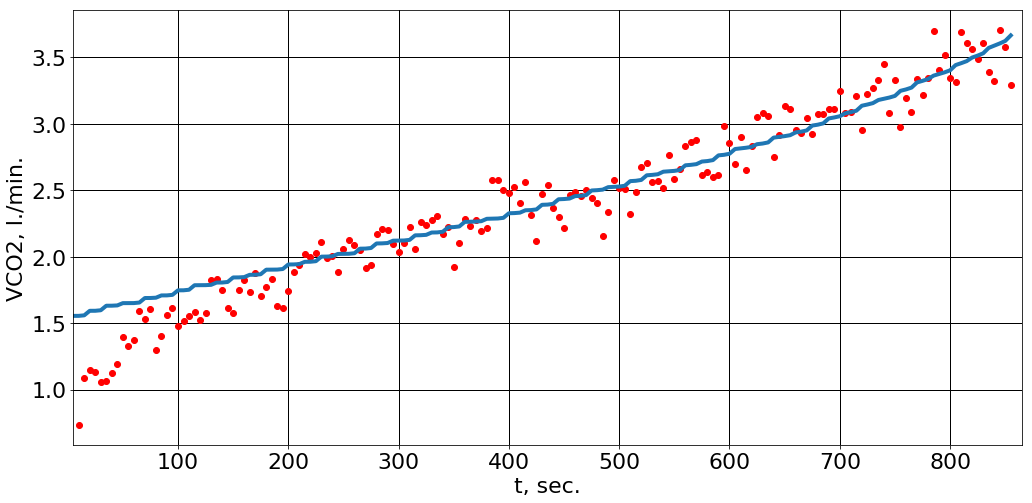
\includegraphics[scale=0.25]{sp102.png}
	\caption{Спортсмен S10. Сравнение экспериментальных и расчетных показателей выделения углекислого газа} 
\end{figure}

\begin{figure}[!ht]
	\centering
	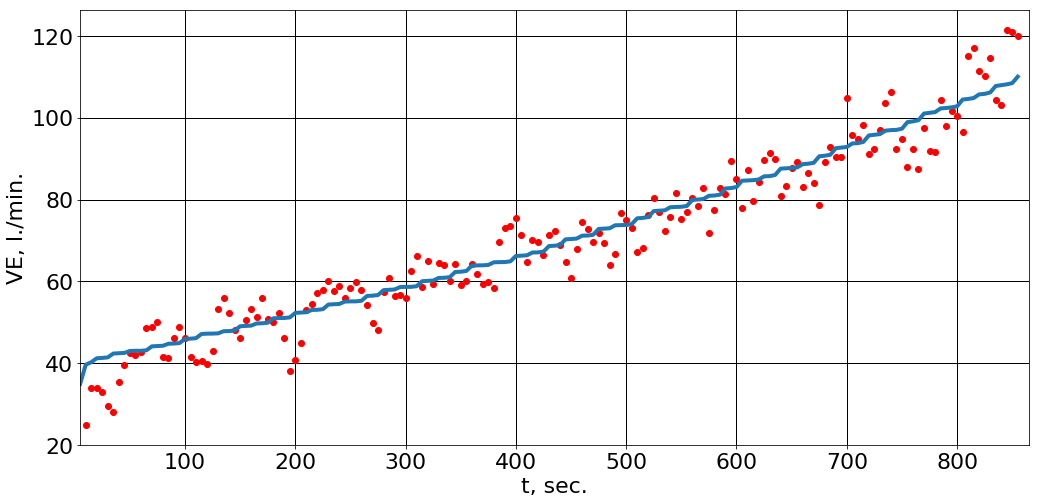
\includegraphics[scale=0.25]{sp104.png}
	\caption{Спортсмен S10. Сравнение экспериментальных и расчетных показателей минутной вентиляции легких} 
\end{figure}

\begin{figure}[!ht]
	\centering
	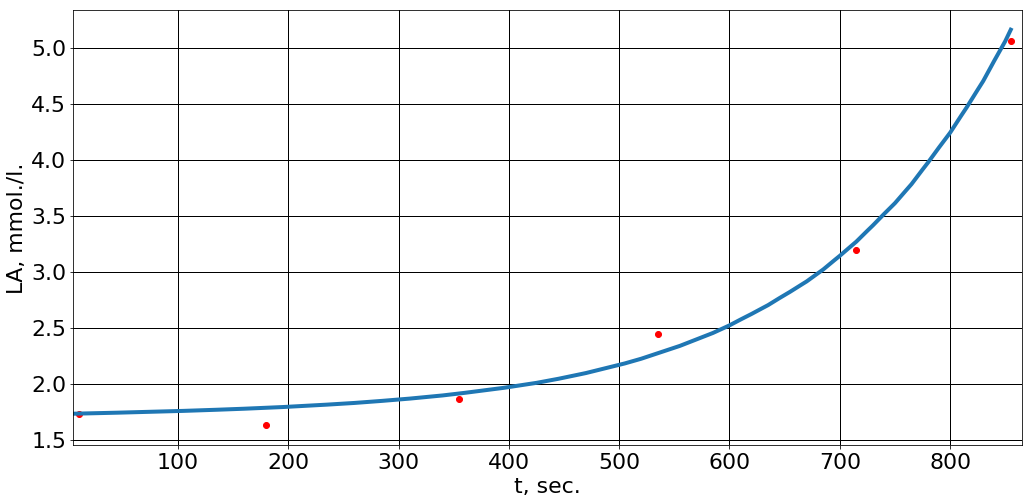
\includegraphics[scale=0.25]{sp103.png}
	\caption{Спортсмен S10. Сравнение экспериментальных и расчетных показателей концентрации лактата} 
\end{figure}